\documentclass[a4paper,USenglish]{lipics}
 
\usepackage{microtype}\bibliographystyle{plain}

\title{Towards Establishing Monotonic Searchability in Self-Stabilizing Data Structures\footnote{This work was partially supported by the German Research Foundation (DFG) within the Collaborative Research Center ``On-The-Fly Computing'' (SFB 901).}}


\author[1]{Christian Scheideler}
\author[2]{Alexander Setzer}
\author[3]{Thim Strothmann}
\affil[1]{Paderborn University\\
  Fürstenallee 11, Paderborn, Germany}
\affil[2]{Paderborn University\\
  Fürstenallee 11, Paderborn, Germany}
\affil[3]{Paderborn University\\
  Fürstenallee 11, Paderborn, Germany}
\authorrunning{C. Scheideler and A. Setzer and T. Strothmann}

\Copyright{Christian Scheideler, Alexander Setzer, and Thim Strothmann}

\subjclass{C.2.4 Distributed Systems}\keywords{Topological Self-Stabilization, Monotonic Searchability, Node Departures}




\usepackage{xcolor}
\usepackage{xspace}
\usepackage{algorithm}
\usepackage[noend]{algpseudocode}
\usepackage{xifthen}
\usepackage{tikz}


\newcommand\mytodo[1]{\textcolor{red}{TODO\ifthenelse{\isempty{#1}}{}{:} #1}}

\algrenewcommand{\algorithmiccomment}[1]{ #1}
\algrenewcommand\algorithmicprocedure{\textbf{action}}


\newcommand{\blp}{\textsc{Build-List+}\xspace}
\newcommand{\srp}{\textsc{Search+}\xspace}
\newcommand{\srpwithoutxspace}{\textsc{Search+}}
\newcommand{\blpp}{\textsc{Build-List*}\xspace}
\newcommand{\srpp}{\textsc{Search*}\xspace}
\newcommand{\bl}{\textsc{Build-List}\xspace}
\newcommand{\linearize}[1]{\textsc{Linearize(\ensuremath{#1})}\xspace}
\newcommand{\introduce}[1]{\textsc{Introduce(\ensuremath{#1})}\xspace}
\newcommand{\tempdelegate}[1]{\textsc{TempDelegate(\ensuremath{#1})}\xspace}
\newcommand{\timeout}{\textsc{Timeout}\xspace}
\newcommand{\search}[1]{\textsc{Search(\ensuremath{#1})}\xspace}
\newcommand{\initsearch}[1]{\textsc{InitiateNewSearch(\ensuremath{#1})}\xspace}
\newcommand{\forwardprobe}[1]{\textsc{ForwardProbe(\ensuremath{#1})}\xspace}
\newcommand{\pnext}[1]{\textsc{Probe(\ensuremath{#1}).Next}\xspace}
\newcommand{\psuccess}[1]{\textsc{ProbeSuccess(\ensuremath{#1})}\xspace}
\newcommand{\pfail}[1]{\textsc{ProbeFail(\ensuremath{#1})}\xspace}
\newcommand{\rvw}{\ensuremath{R(v,w)}\xspace}
\newcommand{\rsp}{\ensuremath{R_s^+}\xspace}
\newcommand{\lsp}{\ensuremath{L_s^+}\xspace}
\newcommand{\rsvw}{\ensuremath{R_s(v,w)}\xspace}
\newcommand{\rv}{\ensuremath{R(v)}\xspace}
\newcommand{\rzvw}{\ensuremath{R_m^0(v,w)}\xspace}
\newcommand{\fdp}{\xspace}
\newcommand{\nidec}{\xspace}



\newcommand{\revandlin}[1]{\textsc{ReverseAndLinearize(\ensuremath{#1})}\xspace} \newcommand{\revandlinREQ}[1]{\textsc{ReverseAndLinearizeREQ(#1)}\xspace}
\newcommand{\revandlinACK}[1]{\textsc{ReverseAndLinearizeACK(#1)}\xspace} 

\newcommand{\templeft}[1][]{\ensuremath{Temp_{L}\ifthenelse{\isempty{#1}}{}{(#1)}}\xspace}
\newcommand{\tempright}[1][]{\ensuremath{Temp_{R}\ifthenelse{\isempty{#1}}{}{(#1)}}\xspace}
 


\begin{document}

\maketitle

\begin{abstract}
Distributed applications are commonly based on overlay networks interconnecting their sites so that they can exchange information. 
For these overlay networks to preserve their functionality, they should be able to recover from various problems like membership changes or faults. 
Various self-stabilizing overlay networks have already been proposed in recent years, which have the advantage of being able to recover from any illegal state, but none of these networks can give any guarantees on its functionality while the recovery process is going on. 
We initiate research on overlay networks that are not only self-stabilizing but that also ensure that searchability is maintained while the recovery process is going on, as long as there are no corrupted messages in the system. 
More precisely, once a search message from node  to another node  is successfully delivered, all future search messages from  to  succeed as well. 
We call this property {\em monotonic searchability}.
 We show that in general it is impossible to provide monotonic searchability if corrupted messages are present in the system, which justifies the restriction to system states without corrupted messages. 
 Furthermore, we provide a self-stabilizing protocol for the line for which we can also show monotonic searchability. 
 It turns out that even for the line it is non-trivial to achieve this property. 
 Additionally, we extend our protocol to deal with node departures in terms of the Finite Departure Problem of Foreback et. al (SSS 2014). 
 This makes our protocol even capable of handling node dynamics.
 \end{abstract}


\section{Introduction}
The Internet has opened up tremendous opportunities for people to interact and exchange information.
 Particularly popular ways to interact are peer-to-peer systems and social networks. 
 For these systems to stay popular, it is very important that they are highly available. 
 However, once these systems become large enough, changes and faults are not an exception but the rule.
Therefore, mechanisms are needed that ensure that whenever there are problems, they are quickly repaired, and all parts of the system that are still functional should not be affected by the repair process. 
Protocols that are able to recover from arbitrary states are also known as \emph{self-stabilizing} protocols.

Since the seminal paper of Dijkstra in 1974~\cite{Dijkstra74}, self-stabilizing protocols have been investigated for many classical problems including leader election, consensus, matching, clock synchronization and token distribution problems.
Recently, also various protocols for self-stabilizing overlay networks have been proposed (e.g., \cite{corona,JRSST09,DolevT2013,JacobRSS2012,DolevK08, AspnesW07,KniesburgesKS12,rechord,DBLP:journals/tcs/BernsGP13}). 
However, for all of these protocols it is only known that they \emph{eventually} converge to the desired solution, but the convergence process is not necessarily \emph{monotonic}. 
In other words, it is not ensured for two points in time  with  that the functionality of the topology at time  is better than the functionality at time .

In this paper, we focus on protocols for self-stabilizing overlay networks that guarantee the \emph{monotonic} preservation of a characteristic that we call \emph{searchability}, i.e., once a search message from node  to another node  is successfully delivered, all future search messages from  to  succeed as well. 
Searchability is a useful and natural characteristic for an overlay network since searching for other participants is one of the most common tasks in real-world networks. 
Moreover, a protocol that preserves monotonic searchability has the huge advantage that in every state, even if the self-stabilization process has not converged yet, the already built topology can already be used for search requests.

As a starting point for rigorous research on monotonic searchability, we will focus on building a self-stabilizing protocol that preserves monotonic searchability for the line graph. 
Although the topology itself is fairly simple, to preserve searchability during the self-stabilization process turns out to be quite challenging. 
Additionally, we study monotonic searchability for the line graph if the node set is dynamic, i.e., nodes are allowed to leave the network.


\subsection{Model}
We consider a distributed system consisting of a fixed set of nodes in which each node has a unique reference and a unique immutable numerical identifier (or short id).
The system is controlled by a protocol that specifies the variables and actions that are available in each node. 
In addition to the protocol-based variables there is a system-based variable for each node called \emph{channel} whose values are sets of messages. 
We denote the channel of node  as  and  contains all incoming messages to . 
Its message capacity is unbounded and messages never get lost.
A node can add a message to  if it has a reference to .
Besides these channels there are no further communication means, so only point-to-point communication is possible.

There are two types of actions. 
The first type of \emph{action} has the form of a standard procedure 
, where  is the unique name of that action,
 specifies the parameter list of the action, and 
specifies the statements to be executed when calling that action. Such actions
can be called remotely. In fact, we assume that every message must be of the
form  where 
specifies the action to be called in the receiving node and 
contains the parameters to be passed to that action call. All other messages
will be ignored by the nodes. Apart from being triggered by messages,
these actions may also be called locally by the nodes, which causes their
immediate execution. 
The second type of action has the form ,
where  and  are defined as above and  is a predicate
over local variables. We call an action whose guard is simply \textbf{true} a
\emph{timeout} action.

The \emph{system state} is an assignment of a value to every variable of each node and messages to each channel. 
An action in some node  is \emph{enabled} in some system state if its guard evaluates to \textbf{true}, or if there is a message in  requesting to call it.
In the latter case the corresponding message is processed (in which case it is removed from ).
An action is \emph{disabled} otherwise. 
Receiving and processing a message is considered as an atomic step.

A \emph{computation} is an infinite fair sequence of system states such that
for each state , the next state  is obtained by executing an
action that is enabled in . This disallows the overlap of action
execution. That is, action execution is \emph{atomic}. We assume \emph{weakly
fair action execution} and \emph{fair message receipt}. Weakly fair action
execution means that if an action is enabled in all but finitely many states
of the computation, then this action is executed infinitely
often. Note that the timeout action of a node is executed infinitely
often. Fair message receipt means that if the computation contains a state
where there is a message in a channel of a node that
enables an action in that node, then that action is eventually executed
with the parameters of that message, i.e., the message is eventually
processed. Besides these fairness assumptions, we place no bounds on message
propagation delay or relative nodes execution speeds, i.e., we allow fully
asynchronous computations and non-FIFO message delivery.
A \emph{computation suffix} is a sequence of computation states past a particular state of this computation. 
In other words, the suffix of the computation is obtained by removing the initial state and finitely
many subsequent states. 
Note that a computation suffix is also a computation.

We consider protocols that do not manipulate the internals of node
references. Specifically, a protocol is \emph{compare-store-send} if the only
operations that it executes on node references is comparing them, storing
them in local memory and sending them in a message. That is, operations on
references such as addition, radix computation, hashing, etc. are not used. In
a compare-store-send protocol, if a node does not store a reference in its
local memory, the node may learn this reference only by receiving it in a
message. A compare-store-send protocol cannot introduce new references to the
system. It can only operate on the references that are already there.

The overlay network of a set of nodes is determined by their knowledge of each other. 
We say that there is a (directed) \emph{edge} from  to , denoted by , if node  stores a reference of  in its local memory or has a message in  carrying the reference of . 
In the former case, the edge is called \emph{explicit} (drawn solid in figures), and in the latter case, the edge is called \emph{implicit} (drawn dashed). 
With  we denote the directed \emph{network (multi-)graph} given by the explicit and implicit edges.
 is the subgraph of  induced by only the explicit edges. 
A \emph{weakly connected component} of a directed graph  is a subgraph of  of maximum size so that for any two nodes  and  in that subgraph there is a (not necessarily directed) path from  to . 
Two nodes that are not in the same weakly connected component are \emph{disconnected}.
We say a node  is to the \emph{left} (\emph{right}, respectively) of a node  if  ().
If there is an edge  between the two, then  is a \emph{left neighbor} (\emph{right neighbor}).
For three nodes  with  (or , respectively), we say a node  is \emph{closer} to  than , if .
If it is clear from the context we sometimes refer to the identifier of a node by dropping the  notation to , e.g., we write  instead of .

In this paper we are particularly concerned with search requests, i.e., \search{v,destID} messages that are routed along  according to a given routing protocol, where  is the sender of the message and  is the identifier of a node we are looking for.
Note that  does not necessarily belong to an existing node , since we also want to model search requests to not existing nodes. 
If a \search{v,destID} message reaches a node  with , the search request \emph{succeeds}; if the message reaches some node  with  and cannot be forwarded anymore according to the given routing protocol, the search request \emph{fails}.
We assume that nodes themselves initiate \search{} requests at will.
Therefore, the \search{destID} action is never explicitly called.

We need some additional notation for our results of Section~\ref{sec:theBLPPAlgorithm}, in which we extend the protocol to handle nodes that want to leave the system.
A node  has a variable  that is read-only. 
If this variable is set to \textbf{leaving}, the node is \emph{leaving}; the node is \emph{staying} if the variable is set to \textbf{staying}.
Note that staying nodes can dynamically decide at any arbitrary state if they want to leave the system by executing a corresponding \emph{leave action}. 
However, a leaving node cannot switch back to staying.
The ultimate goal of a leaving node is to depart from the system.
There is one special command that is important for the study of leaving nodes: \textbf{exit}. 
If a node executes \textbf{exit} it enters a designated \emph{exit state} and all remaining edges to or from that node are deleted. 
We call such a node \emph{gone}. 
A node that is not gone is called \emph{present}.
For a gone node all actions are disabled, in particular it will not execute the timeout action regularly.

\subsection{Problem Statement}

A protocol is \emph{self-stabilizing} if it satisfies the following two properties.
\begin{description}
\item[\emph{Convergence:}] starting from an arbitrary system state, the protocol is guaranteed to arrive at a legitimate state.
\item[\emph{Closure:}] starting from a legitimate state the protocol remains in legitimate states thereafter.
\end{description}
A self-stabilizing protocol is thus able to recover from transient faults regardless of their nature. 
Moreover, a self-stabilizing protocol does not have to be initialized as it eventually starts to behave correctly regardless of its initial state. 
In \emph{topological self-stabilization} we allow self-stabilizing protocols to perform changes to the overlay network, resp.~. 
A legitimate state may then include a particular graph topology or a family of graph topologies.

In this paper we want to build a self-stabilizing protocol for the \emph{linearization problem}, i.e., the nodes are sorted by identifiers and each node stores only two references: its closest successor and its closest predecessor.
From a global point of view, the nodes build a \emph{line graph} topology.
Of course, searching is easy once a legitimate state has been reached.
However, searching reliably during the stabilization phase is much more involved.
We say a (self-stabilizing) protocol satisfies \emph{monotonic searchability} according to some routing protocol  if it holds for any pair of nodes  that once a \search{v,id(w)} request (that is routed according to ) initiated at time  succeeds, any \search{v,id(w)} request initiated at a time  will succeed.
We do not mention  if it is clear from the context.
A protocol is said to satisfy \emph{non-trivial} monotonic searchability if it satisfies monotonic searchability and in every computation of the protocol there is a suffix such that for each pair of nodes  for which there is a path from  to  in the target topology \search{v,id(w)} requests will succeed.

Furthermore, we give a self-stabilizing protocol that satisfies non-trivial monotonic searchability, solves the linearization problem and solves the \emph{Finite Departure Problem} of~\cite{departure1}. The following problem statement is adapted from~\cite{KoutsopoulosSS15}:
\begin{description}
\item[\emph{Finite Departure Problem} (\fdp)]: In case the \textbf{exit} command is available, eventually reach a system state in which (i) every staying node is awake, (ii) every leaving node is gone and (iii) for each weakly connected component of the initial network graph, the staying nodes in that component still form a weakly connected component.
\end{description}
Consequently, a leaving node  should \emph{safely} execute \textbf{exit}, i.e., the removal of  and its incident edges from  does not disconnect any present nodes and does not violate searchability.


\subsection{Related work}


The idea of self-stabilization in distributed computing was introduced in a classical paper by E.W. Dijkstra in 1974~\cite{Dijkstra74}, in which he looked at the problem of self-stabilization in a token ring. 
In order to recover certain network topologies from any weakly connected state, researchers started with simple line and ring networks (e.g.~\cite{ShakerR05,self-stabilizing-list,self-stabilizing-list2}.
Over the years more and more network topologies were considered, ranging from skip lists and skip graphs~\cite{corona,JRSST09}, to expanders~\cite{DolevT2013}, Delaunay graphs~\cite{JacobRSS2012}, hypertrees and double-headed radix trees~\cite{DolevK08, AspnesW07}, small-world graphs~\cite{KniesburgesKS12} and a Chord variant~\cite{rechord}. 
Also a universal algorithm for topological self-stabilization is known~\cite{DBLP:journals/tcs/BernsGP13}.

Close to our work is the notion of \emph{monotonic convergence} by Yamauchi and Tixeuil~\cite{YamauchiT10}. A self-stabilizing protocol is monotonically converging if every change done by a node  makes the system approach a legitimate state and if every node changes its output only once. 
The authors investigate monotonically converging protocols for different classic distributed problems (e.g., leader election and vertex coloring) and focus on the amount of non-local information that is needed for them.

Our study of the \emph{Finite Departure Problem} is heavily inspired by~\cite{departure1}, in which the authors propose the aforementioned problem to study graceful departures of nodes in a self-stabilizing setting, i.e., nodes that want to leave a distributed system should decide when they can leave without affecting weak connectivity of the topology. 
They conclude that in general it is not possible to solve the \fdp. 
However, with the use of distributed oracles (which are specialized failure detectors~\cite{ChandraT96}) the authors propose a protocol that solves the problem and arranges the nodes in a line. 
Additionally, they can show that oracles are not needed if the problem is transformed into a non-decision variant. 
In~\cite{KoutsopoulosSS15} the idea is generalized to a protocol framework that solves the \fdp without being reliant on a certain topology and is thereby combinable with most existing overlay protocols.

\subsection{Our contribution}
To the best our knowledge, this paper presents the first attempt to have stricter requirements towards the self-stabilization process in topological self-stabilization.
We define and study \emph{monotonic searchability}, which captures a typical use case for overlay networks, i.e., searching other nodes.
More formally, we want to guarantee for a self-stabilizing topology that once a search message from node  to another node  is successfully delivered, all future search messages from  to  succeed as well.
We focus on studying non-trivial monotonic searchability for the list topology.
First, we show that in general it is impossible to provide non-trivial monotonic searchability from any initial system state, due to the presence of certain initial messages.
This justifies to study searchability only for so-called \emph{admissible system states} in which  these messages are not present anymore, as long as the protocol gurantees convergence to these states.
We give a self-stabilizing list protocol and an appropriate search protocol that achieve the desired goal and prove their correctness.
Moreover, we broaden the elaborateness of the problem statement, by allowing nodes to leave the line topology, i.e., solving the Finite Departure Problem in addition to the aforementioned problems. 
Also for this combination of problems we present suitable protocols and prove their correctness. 

\section{Preliminaries}
\label{sec:preliminaries}

Since gone nodes will never execute any action, we only consider initial states in which all nodes are present. 
We also restrict the initial state to contain only a finite number of messages that can trigger actions specified by our protocol, since other messages are ignored by the nodes. 
Finally, we do not allow the presence of references that do not belong to a node in the system.
From now on, an initial system state satisfies all of these constraints.

The following propositions are restatements of results in~\cite{corona} and imply further necessary conditions on initial system states.
\begin{enumerate}
\item If a compare-store-send program solves the linearization problem, each computation starts in a weakly connected initial state.
\item If a compare-store-send program solves the linearization problem, each computation starts in a state in which all references belong to present nodes.
\end{enumerate}

A \emph{message invariant} is a predicate of the following form:
If there is a message  in the incoming channel of a node, then a predicate  must hold.
A protocol may specify one or more message invariants.
An arbitrary message  in a system is called \emph{corrupted} if the existence of  violates one of the message invariants.
A state  is called \emph{admissible} if there are no corrupted messages in .
We say a protocol \emph{admissible-message satisfies} a property if the following two conditions hold: (i) in computations in which every state is admissible, it satisfies the property, and (ii) starting from any initial state, there is a computation suffix in which every state is admissible.
A protocol \emph{unconditionally satisfies} a property if it satisfies this property starting from any state.

With this notion in mind, we can show that admissible-message satisfaction is necessary for non-trivial monotonic searchability for any routing algorithm .

\begin{lemma}\label{lem:admissible_message_necessary_for_monotonic_searchability}
If a compare-store-send self-stabilizing protocol satisfies non-trivial monotonic searchability then this protocol must be admissible-message satisfying.
\end{lemma}
The structure of the proof is as follows: we consider an arbitrary unconditionally satisfying protocol and show that it does not satisfy monotonic searchability by creating a bad instance for this protocol.
In particular, we exploit that our model does not ensure FIFO delivery of messages.

\begin{proof}
  Assume there is a compare-store-send self-stabilizing protocol that unconditionally satisfies non-trivial monotonic searchability.
  First of all, note that if it violates only the second condition of admissible-message satisfiability, then there are computations in which monotonic searchability is never satisfied, implying that it cannot satisfy non-trivial monotonic searchability.
  Thus, assume that the first condition is violated, i.e., the protocol satisfies the property in computations with arbitrary message, regardless of any invariants.
  Consider the network given in Figure~\ref{fig:no_corrupt}.
  \begin{figure}[h]
    \centering
 	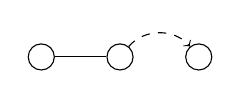
\begin{tikzpicture}
		\node(u)[circle,draw=black] at (0,0) {};
		\node(v)[circle,draw=black] at (1,0) {};
		\node(w)[circle,draw=black] at (2,0) {};
		\draw (u) -- (v);
		\draw[dashed,->] (v) to[out=50,in=-230] (w);
	\end{tikzpicture}
	\caption{Instance for this proof.}\label{fig:no_corrupt}
 \end{figure}
 
 The implicit edge  is in .
 We carry out the proof as a game between the protocol and an adversary: based on the decisions of the protocol,  the adversary may decide on the delivery speed of messages, and imitate additional messages at each node.
 The latter is possible since nodes can not distinguish between these messages and messages from an initial state that have not been received yet.
 Furthermore, the adversary may set the initial state of the nodes.
 
 At first, we issue a  request in  that we denote by  in the following.
 We argue that the adversary can force  to forward  to .
 Therefore note the following:
 \begin{enumerate}
  \item As long as  does not receive any further messages,  does not know any other node, so  is the only possible next hop for .
  \item If  tries to wait for a certain amount of time before sending , the adversary simply halts the system for that time, i.e., no messages are delivered in that timeframe and the system state stays the same.
  \item If  requires the receipt of another message in order to forward , the adversary imitates this message at .
  \item If  relies on its internal state to forward , the adversary changes the initial state of  such that it does not forward any message, which contradicts the assumption that non-trivial monotonic searchability is satisfied.
  Therefore,  must not rely on its state to forward .
  \item There are no other conditions that  can wait on.
 \end{enumerate}
 Therefore,  will send out  to  eventually. At the point in time when  does so, we issue a second  request in .
 For similar reasons as stated above,  must be sent to  at some point in time as well.
 
 Since both messages are in  and the adversary is allowed to decide message speeds, it lets  receive  first.
 Node  has no explicit edge to  and the adversary can enforce that the implicit edge  will not be received by  until  handles . Therefore  must be answered with ``FAIL'' at some point in time (since the  cannot be forwarded anymore) and  will be informed about that.

 Next, the adversary causes the edge  to arrive at .
 Since the protocol must stabilize to the line, at some point in time, the edge  will be established.
 Until then, the adversary withholds message  in .
 Afterwards, when  arrives at , it can be forwarded to  and thus correctly served.
 
 Therefore, message  succeeds, whereas message  that was sent after message  fails.
 This is a contradiction to the assumption that the protocol achieves non-trivial monotonic searchability. 
\end{proof}


Consequently, to prove non-trivial monotonic searchability for a protocol (according to a given routing protocol ) it is sufficient to show that: (i) the protocol has a computation suffix in which every state is admissible and (ii) the protocol guarantees non-trivial monotonic searchability according to  in admissible states.

For the \fdp, it was shown in~\cite{departure1}, there is no distributed protocol within our model that can decide when it is safe for a node  to leave the system and thereby solve the \fdp.
The authors circumvent this impossibility result with the help of oracles.
In general, an \emph{oracle} is a predicate that depends on the current system state and the node calling it. 
In the context of the \fdp, an oracle is supposed to advise a leaving node when it is safe to execute \textbf{exit}.
We use the oracle \nidec as introduced in~\cite{departure1} in order to solve the \fdp. 
\nidec evaluates to \textbf{true} for a node  calling it, if no node  has a reference to  in its local memory or in a message in  and if  is empty. For an in depth discussion of oracles for the \fdp, we refer the reader to~\cite{departure1,KoutsopoulosSS15}. 


\section{The \blp and the \srp protocols}
\label{sec:blpAlgorithm}

In this section, we present the \blp protocol and the \srp protocol. \blp solves the linearization problem and is admissible-message satisfying non-trivial monotonic searchability according to \srp.
Note that any protocol satisfying non-trivial monotonic searchability must be admissible-message satisfying as shown in Section~\ref{sec:preliminaries}.
This section is organized as follows: 
First, we describe \blp and \srp in detail (Subsection~\ref{subsec:blp_desription}).
Then, we prove that the \blp protocol solves the linearization problem (Subsection~\ref{sec:self_stabilization_proof}).
Last, we prove that the \blp protocol satisfies non-trivial monotonic searchability according to \srp (Subsection~\ref{sec:monotonic_searchability_proof}).
From now on we drop the "according to \srpwithoutxspace" clause, since we only consider searchability for \srp.

\subsection{Description of \blp and \srp}
\label{subsec:blp_desription}
The \blp Protocol builds upon the protocol introduced in~\cite{self-stabilizing-list} that solves the linearization problem.
For this protocol, every node only keeps a single left and right neighbor. 
If a node  receives a reference of a node  with  (, respectively),  either saves  as its new right (left) neighbor if  is closer to  than the current right (left) neighbor  and delegates the reference of  to  or (in case  is not closer),  is not saved and delegated to .
Here, \emph{delegation} means that the reference of a node is sent in a message to another node and not kept in the local memory.
A natural (local) search protocol for this topology is to always forward search requests to the neighbor closest to the desired target node, or to abort the search request in case no such neighbor exists.
Note that these easy and elegant protocols cannot guarantee monotonic searchability due to three simple facts: (i) due to delegation, it is possible that an explicit edge  is replaced by an explicit edge  and an implicit edge , (ii) consequently,  are not in the same weakly connected component in  (even though they were before delegation) and (iii) searchability is defined for .

The \blp protocol introduces the following changes in order to satisfy monotonic searchability:
Instead of having a single left and right neighbor, a node  has sets of neighbors  and  (that it sorts implicitly according to id).
In the following, whenever we use the notation /, we refer to these sets of a node .
The main principle that we use is that every node  does not delegate any edge to a node  stored in  or  directly.
Instead it first introduces (using \introduce{v,w}) this node to another node , waits for an acknowledgement that the edge has been added to  or  (which is basically the \linearize{v} message) and then delegates the edge to a node closer to  (using \tempdelegate{v}).
More specifically, whenever a node  has multiple neighbors to one side, it does not delegate edges to the closest neighbor directly, but does the following.
W.l.o.g. assume that it has multiple neighbors  to the right with .
In the \timeout action  introduces  to , with an \introduce{w_i,u} message.
Thereby,  knows that it got the reference from , saves the reference to  directly, sends a \linearize{w_i} message back to  and a \tempdelegate{u} to itself (the latter is only to preserve connectivity).
Node  can now react to that \linearize{w_i} message, by deleting  from its memory and sending the reference to the closest node to the left of  in  (which is not necessarily  anymore). 
Thereby,  preserves a path of explicit edges between  and .
Additionally,  sends its own reference to the closest neighbors with a  message who turn this into a \tempdelegate{u} message.
In general, the \tempdelegate{u} action is used to delegate an implicit edge to a node  into one direction (i.e., to the left or to the right) as long as there is a node between the current node and  in  or .
Note that implicit edges are not used for search, thus we do not have to apply the principle of introducing first and delegating afterwards for this kind of edges.
However, we have to delegate in order to preserve connectivity and to stabilize to the line eventually.
Note that, even though a node has temporarily more references than necessary for the final line topology our protocol still eventually stabilizes to the line, as we will show later.
The pseudocode for all \blp actions is given in Listing~\ref{algo:blp}.
Note that a node refers to itself with the expression .
Additionally, keep in mind that the timeout action is the only action that is not triggered as a result of another action.
Instead, is triggered regularly.

\begin{lstlisting}[mathescape=true,float=*,caption=\blp protocol,label=algo:blp]

 for all 
   send  to 
 //Let  with  
 for all  with 
   send  to 
 //Let  with     
 for all  with 
   send  to 
 send  to 
 send  to 

 
 if()
   if{}
     
     send  to 
     send  to 
   else //
     send  to 
 else if() 
   //Analogous to the previous case.
    

 send  to 
 if()
   if()
     
     if()
       
       
       send  to 
 else if() 
   //Analogous to the previous case. 
 

 if()
   if()
      
   else //
     
     if()
       
     else if()
       send  to 
 else if{} 
   //Analogous to the previous case. 

\end{lstlisting}


The \srp protocol works as follows:
Whenever the \initsearch{destID} action is called at a node ,  creates a new \search{u,destID} message and starts to periodically initiate \forwardprobe{u,destID, \{u\}, self.seq} messages that it sends to itself. 
In the following, assume  (the other case is analogous).
Each \forwardprobe{} message has a set of nodes, called  attached to it, which contains the nodes the message will visit in its future. 
It also has a counter  attached to it whose meaning we will explain later.
Whenever a \forwardprobe{u,destID, Next, seq} message is at a node ,  removes itself from  and adds all its right neighbors  with  to . 
Then it forwards the \forwardprobe{u,destID, Next, seq} message to the node with minimal id in .
If a \forwardprobe{u,destID, Next, seq} message arrives at a node  with , it directly responds with a \psuccess{destID,seq, v} message to .
However, if  is empty at a node  with  after  has added the aforementioned right neighbors, the \forwardprobe{} message is answered with a \pfail{destID,seq} message.
In any case, as soon as  receives the response, it acts accordingly: If the answer to a \forwardprobe{u,destID,Next,seq} message is a \pfail{destID,seq} message, it drops the corresponding \search{u,destID} message completely.
If the answer is \psuccess{destID,v}, \search{u,destID} messages waiting at  are directly sent to .

Note that if additional \search{u,destID} messages are created at  while  is still waiting for an answer to an earlier initiated \forwardprobe{u,destID}, these requests simply wait together with the previous request (realized by simple  field) and are aborted or sent as soon as the \pfail{destID} or \psuccess{destID,v} response arrives at , (i.e., search requests to the same destination are sent out in batches if possible).
Furthermore, note that nodes do not memorize whether they have already sent \forwardprobe{} messages to a certain destination. Due to corrupt initial states, this knowledge could be wrong and nodes relying on this knowledge would wait forever.
Therefore, nodes periodically send \forwardprobe{} messages, instead of only once.
Note that because we make no assumptions on the message delivery speed and channels are not FIFO, it is possible that \pfail{} messages arrive at a node  that are answers to \forwardprobe{} messages initiated long ago.
However, in the meantime, there might have been successful responses.
To deal with this, each node  stores a sequence number counter .
Whenever \initsearch{destID} is executed by  and there is no \search{u,destID} that waits for an answer to a \forwardprobe{u,destID, Next, seq} message,  increments , stores the new  value in an entry for  and always attaches the current sequence number () to each \forwardprobe{} message  sends.
Responses to probes (success and failure) sent by  also contain this sequence number.
Whenever a response is sent back to ,  checks whether the sequence number in this message is at least the sequence number stored for .
If not, it simply drops the message, since in that case, the answer belongs to a \forwardprobe{} message sent for an earlier batch of \search{u,destID} messages that have already been processed.
The complete pseudocode for \srp is given in Listing~\ref{algo:search}.


\begin{lstlisting}[mathescape=true,float,caption=\srp protocol,label=algo:search]

 create new message 
 if()
   
   
   
 //Store the messages to  
  


 if()
   if()
     for all 
       send  to 
   send  to 
   send  to 
 else //
   if()
     
     if()
       send  to 
       send  to 
     else //
       
       if()
         send  to 
       else if()
         
       send  to 
   else if() 
     //Analogous to the previous case.
 

 if()
   /* The message belongs to currently  
    * stored search requests to . */
   send all  to 
   
 send  to 
 

 if()
   /* The message belongs to currently  
    * stored search requests to . */
   
\end{lstlisting}


In order to not unnecessarily blow up the pseudocode, we intentionally left out a sanity check for each node, i.e., before executing each action, each node  makes sure that  only contains nodes  with  and that  only contains nodes  with .
If this is not the case for some node ,  rearranges the reference to  accordingly.
This way, in every computation, the following lemma holds:

\begin{lemma}\label{lem:left_and_right_are_what_they_say}
  For every node  it holds: For all , , and for all , .
\end{lemma}


\subsection{\blp solves the linearization problem}\label{sec:self_stabilization_proof}
In this section, we prove the following theorem:
\begin{theorem}\label{thm:blp_solves_linearization}
 \blp is a self-stabilizing solution to the linearization problem. 
\end{theorem}
We prove the theorem in three steps: 
First, we show that starting from any initial state in which  is weakly connected,  will always be weakly connected.
Second, we show that starting from any initial state, there will be a state in which  will be a supergraph of the line graph and that the explicit edges corresponding to the line will never be removed.
Third, we prove that all superfluous explicit edges will eventually vanish.


The first step is represented by the following lemma:
\begin{lemma}\label{lem:NG_remains_weakly_connected}
 If a computation of \blp starts from a state where  is weakly connected then in every state,  remains weakly connected.
\end{lemma}

\begin{proof}
  First, note that in every action whenever a message with a reference to a node  is received by a node  then either  is added to the set  or  or a new message is created with  as a parameter and sent to a node .
  Thus, the implicit edge  is replaced by a path .
  
  Furthermore, the only action for that removes a reference to  from one of the sets  or  is the \linearize{v} action.
  However, in \linearize{v}, if  is removed from  or ,  is also introduced to a node  in  or .
  Thus, the edge  is replaced by a path  in this case, too.
\end{proof}

For the second step of the proof of the theorem, we introduce the notation  and .
Furthermore, let  for two nodes  and  denote the hop distance in the (ideal) line topology between  and .
We define  for a node  as  if  or as  if ; we define  analogously for .
With this, we define a potential function  where  are all nodes ordered by their id increasingly.
Notice that  is bounded from above by  and from below by .
Also notice that according to the protocol,  () can only change if  puts a node closer to  than  () into  ().
Thus,  never increases.
We define the \emph{closest neighbor graph} as the graph  where  is the set of all nodes and  iff .
Furthermore, we say an edge is \emph{temporary} if it is an implicit edge due to a \tempdelegate{} message.
 All other types of implicit edges are called \emph{non-temporary}.
One can show the following:
\begin{lemma}\label{lem:closest_neighbor_graph_bidirected_and_strongly_connected}
 Assume there is a system state such that  does not decrease in any further step of the computation.
 Then  is bidirected and strongly connected.
\end{lemma}
We prove this lemma step-by-step, starting with the following lemma:
\begin{lemma}\label{lem:closest_neighbor_graph_bidirected}
 Assume a system state such that  does not decrease in any further step of the computation.
 Then  is bidirected.
\end{lemma}

\begin{proof}
 Assume for contradiction there exists an edge  such that  and w.l.o.g. assume .
 This implies  and .
 Since  does not change any more,  will remain  and eventually by the fair action execution assumption, \timeout will be executed in  and  will send an \introduce{x,\bot} to , which, by the fair message receipt assumption, will be eventually delivered to .
 This implicit edge will turn into a temporary edge .
 Note that if  or , then, according to the protocol and because ,  will be replaced by  causing  to decrease, which contradicts to the initial assumption.
 Therefore,  and  must hold.
 According to the protocol,  will be delegated (first to , then possibly further) until it reaches at a node  with  .
 Here similar arguments as above yield a contradiction. 
 Thus,  must be bidirected.
\end{proof}
The definition of a closest neighbor graph and Lemma~\ref{lem:left_and_right_are_what_they_say} imply the following:
\begin{corollary}\label{cor:only_topology_is_line}
 If  is bidirected and disconnected, every connected component forms a line.
\end{corollary}
To show that  is also strongly connected, we need two additional lemmata.
We start with the following:
 \begin{lemma}\label{lem:non_temporary_will_become_expl_or_temporary}
  Assume that in a state of the computation of \blp  is bidirected and disconnected.
  If there is a non-temporary edge  with  for a connected component , then eventually either there will be an explicit or a temporary edge  with  and  or  will decrease.
 \end{lemma}
 
 \begin{proof}
W.l.o.g., assume .
First of all, note that according to the protocol, if the graph  changes,  must decrease.
Since in that case we are done, in the following we assume that  will never change.
Furthermore, by Corollary~\ref{cor:only_topology_is_line}, the connected components of  form a line.
We now make a case distinction over all possible types of :
 \begin{enumerate}
  \item  is an implicit edge from a \forwardprobe{m} message in which  or  and . 
	Then once the message is received,  will be turned into a temporary edge and the claim follows.
   \item  is an implicit edge from a \forwardprobe{m} message in which  and .    
	Consider the state in which this message is received and the corresponding action is executed.
	Then  is updated according to the protocol.
	If  is empty after this operation, a temporary edge  is established and the claim holds.	
	Otherwise, let  after the update.
	Note that if , we have two sub-cases: Either  or .
	In the former case,  will be added to , causing  to decrease, and the claim holds.
	In the latter case, due to the way  was updated,  must hold.
	Applying the previous arguments recursively yields that the message will, at some point in time, reach at a node  where either  or  after the update.
	In this case, a temporary edge  will be established.
	\\
	Now, consider the case .
	Again, we have two sub-cases: Either  or .
	In the former case, since the protocol establishes the temporary edge , the claim follows.
	In the latter case, the message will be forwarded to .
	According to the protocol, for  after the update of , it holds . Thus, this case reduces to the other case above.
  \item  is an implicit edge from a \forwardprobe{m} message in which  and .    
	This case is analogous to the previous one.
  \item  is an implicit edge from a \forwardprobe{m} message in which  and .    	
	Note that in this case if a \forwardprobe{m} message is delegated from a node  to a node , then a temporary edge  is also established.
	Then either  directly proving the claim, or .
	Observe that each \forwardprobe{m} message can only be delegated from a node  to a node  once.
	Thus, either starting from the first or the second step, whenever a \forwardprobe{m} message is delegated from a node  to a node , then .
	Furthermore, note that the protocol assures , i.e.,  as well.
	The only case when a \forwardprobe{m} message is no longer delegated is if  is empty (in which there is nothing left to prove), or when  for a node .
	In the latter case, for each node remaining in , a temporary edge is created.
  \item  is an implicit edge from a \forwardprobe{m} message in which  and .
	This case is analogous to the previous one.
  \item  is an implicit edge from a \psuccess{} (in which  is ) message and a temporary edge  will be established.
  \item  is an implicit edge from an \introduce{} message.
	Note that according to the protocol, all edges in an \introduce{} message are added either as explicit edges or as temporary edges.
  \item  is an implicit edge from a \linearize{} message and  will be turned into a temporary edge.
 \end{enumerate} 
\end{proof}
\begin{lemma}\label{lem:temporary_will_shorten_or_phi_will_decrease}
  Assume that in a state of the computation of \blp  is bidirected and disconnected.
  If there is an explicit or a temporary edge  with  and  for a connected component , then eventually there will be an explicit or temporary edge  with  and , or  will decrease.
 \end{lemma}

\begin{proof}
  W.l.o.g., assume .
  First, assume  is an explicit edge. 
  If , we have a contradiction to the assumption  and .
  Thus  must hold. 
  In this case, in \timeout a new edge  with  will be introduced and the claim will hold.
  Second, assume that  is an implicit edge from a \tempdelegate{} message. 
  Then either  and  turns into an explicit edge and  becomes , causing  to decrease, or a \tempdelegate{v} message is sent to  resulting in a shorter edge .
  This completes the proof of the second claim.
\end{proof}

We are now ready to prove \textbf{Lemma~\ref{lem:closest_neighbor_graph_bidirected_and_strongly_connected}}:
\begin{proof}
  Assume there is an initial state in which  does not decrease anymore.
  Furthermore, assume that the closest neighbor graph  is disconnected.
  Firstly, Lemma~\ref{lem:closest_neighbor_graph_bidirected} guarantees that  is bidirected.
  Furthermore, by Lemma~\ref{lem:NG_remains_weakly_connected}, there must be at least one (implicit or explicit) edge  between a connected component  and another connected component.
  Together with Lemma~\ref{lem:non_temporary_will_become_expl_or_temporary} this implies that at some point there must be a temporary or explicit edge  with  and .
  However, then Lemma~\ref{lem:temporary_will_shorten_or_phi_will_decrease} can be applied.
  Since there is only a finite number of times that there can be a shorter edge, at some state,  must decrease, yielding a contradiction.
  Thus  must be weakly connected.
  Note that Lemma~\ref{lem:closest_neighbor_graph_bidirected} implies that  is also strongly connected, yielding the claim of Lemma~\ref{lem:closest_neighbor_graph_bidirected_and_strongly_connected}.
\end{proof}
Note that since  can never increase and since  is bounded from below,  can only decrease for a finite number of states.
After that, the conditions of Lemma~\ref{lem:closest_neighbor_graph_bidirected_and_strongly_connected} are fulfilled.
This lemma and Corollary~\ref{cor:only_topology_is_line} imply the following corollary:
\begin{corollary}\label{cor:explicit_edge_graph_will_become_supergraph}
 For any computation of \blp, there is a state in which the graph formed by the explicit edges is a supergraph of the line topology.
\end{corollary}
For the third step of the proof of the theorem, we have the following lemma:
\begin{lemma}\label{lem:superfluous_edges_will_vanish}         
 If a computation of \blp contains a state in which  is a supergraph of the line topology, then there will be a suffix in which  is the line topology and no new explicit edges will ever be created again.
\end{lemma}

\begin{proof}
    For the proof, we introduce the following notatation: We say an implicit edge  is \emph{right-relevant} if  and the implicit edge  is due to a  message in  for .
    Accordingliy, we say an edge  is \emph{left-relevant} if  and the implicig edge  is due to a  message in  for .
    Additionally, we call an explicit edge  \emph{superfluous} if .


  Consider the state in which the graph formed by the explicit edges is a supergraph of the line topology.
  First of all, notice that according to the protocol, an explicit edge  that belongs to the line topology will never be removed (because this would require a node  to get acquainted with a node  that is closer than  or  which is not possible).
  In addition, notice that according to the protocol, in every state (right-/left-)relevant edges are the only implicit edges that can be turned into an explicit edge any more.
  Notice that a right-relevant edge  can only be created by a node  with a superfluous explicit edge to .
  Thus, for every node  it holds: if there is no node  with a relevant or superfluous edge , then there will never be a relevant or superfluous edge  with  again.
  
  Consider the leftmost node  that either has at least one right-relevant edge or at least one superfluous right neighbor.
  Note that once all right-relevant edges have been received by , then no node  will ever add a superfluous right neighbor again.
  Furthermore, notice that right-relevant edges will be turned into explicit edges upon receipt.
  Now, for every superfluous right neighbor  of ,  will send an \introduce{v,u} to some node .
  Each of these will eventually be received and, according to the protocol, be answered with a \linearize{v} message at .
  This will cause  to delegate  to a node .
  After the last superfluous edge has been delegated, no node  will ever have a superfluous right neighbor again.
  
  Continuing this approach, we can show that all superfluous right neighbors will eventually vanish.
  Using analogous arguments, we can also show that all superfluous left neighbors will eventually vanish.
  Thus, the lemma follows.
\end{proof}
Note that Corollary~\ref{cor:explicit_edge_graph_will_become_supergraph} and Lemma~\ref{lem:superfluous_edges_will_vanish} imply that \blp converges to the list.
Moreover, Lemma~\ref{lem:superfluous_edges_will_vanish} yields the closure property.
This finishes the proof of Theorem~\ref{thm:blp_solves_linearization}.

\subsection{\blp satisfies non-trivial monotonic searchability}\label{sec:monotonic_searchability_proof}
In this subsection we prove the following theorem:
\begin{theorem}\label{thm:blp_guarantees_monotonic_searchability}
 \blp admissible-message satisfies non-trivial monotonic searchability according to \srp.
\end{theorem}


We start with some preliminaries.
First we define  as the set of all nodes  with  for which there is a directed path from  to  consisting solely of explicit edges  with .
Furthermore, we define .
In addition, we define  as the set of all nodes  with  for which there is a directed path from  to  consisting solely of explicit edges  with .
For a set ,  and .
Accordingly,  and .

Moreover, we define a state as admissible if the following message invariants hold:
\begin{enumerate}
 \item If there is an \introduce{v,w} message with  in , then , and  (or ).
 \item If there is a \linearize{v} message in , then there is a node  with  and  if  (or  and  if ).
 \item If there is a \forwardprobe{source,destID,Next,seq} message in , then
    \begin{enumerate}
      \item  and  and  
      (alternatively  and  and ).
      \item  and  (or  and ).
      \item if  exists such that  and  and  (or  and ) then for every admissible state with ,  ().
    \end{enumerate}
 \item If there is a \psuccess{destID, seq, dest} message in , then  and  if  (or  if ).
 \item If there is a \pfail{destID, seq} message in , then either there is no node with id , or for every admissible state with ,  (and ), where  such that .
 \item If there is a \search{v, destID} message in , then  and  if  (or  if ).
\end{enumerate}



\begin{lemma}\label{lem:once_admissible_always_admissible}
 If in a computation of \blp, there is an admissible state, then all subsequent states are admissible.
\end{lemma}

In order to prove Lemma~\ref{lem:once_admissible_always_admissible}, we need the following lemmata:
\begin{lemma}\label{lem:once_first_two_invariants_hold_then_always}
 If in a computation of \blp, the first two invariants hold, then in all subsequent states the first two invariants will hold.
\end{lemma}
\begin{proof}
 Assume there is a state  in which the first two invariants hold and such that in the (direct) subsequent state  one of the first two invariants does not hold.
 Obviously, this can only be due to one of the following three reasons:
 First, a new \introduce{v,w} message with  was sent to a node  with  (and ) in .
 Second, a new \linearize{v} message was sent to a node  in , but there is no node  with  and  (or  and ).
 Third, a node  was removed from a set  (or ).
 We show that all three cases cannot happen.
 
 For the first case, notice that according to the protocol, the only occasion when an \introduce{v,w} message with  is sent is in the \timeout action of a node .
 Here, it is only sent to nodes in  (or ) and only with a first parameter .
 
 For the second case, notice that according to the protocol, the only occasion when a \linearize{v} message is sent to a node  is in an \introduce{v,w} action at a node .
 This must have been triggered by an \introduce{v,w} message with .
 Thus, before the action was executed, by the first invariant,  (or ) and  were both fulfilled.
 This implies that there must be a node , i.e.,  such that  or  (or a node , i.e., , such that  or ).
 During the execution of the action,  was added to  (or ), which implies  (or ).
 
 For the third case, note that a node  is only removed from  (or ) if the \linearize{y} action has been executed in  between  and .
 However, by the second invariant, there must be a node  with  and  (or  and ).
 Thus, after the removal,  still holds.
 
 Therefore, in all three cases the first two invariants cannot be violated and have to hold in , too.
\end{proof}


\begin{lemma}\label{lem:R_grows_monotonically}
  If there is a state in which the first two invariants hold, and  (), then in every subsequent step,  ().
\end{lemma}
\begin{proof}
We only consider the case , as  is completely analogous.

Obviously, adding additional edges does not remove elements from .
The only action that delegates away an explicit edge  stored in  for some nodes  (and hence could remove nodes from ) is the \linearize{} action if .
Therefore, consider an arbitrary \linearize{z} action executed by .
Note that since we assumed that the first two invariants hold, right before \linearize{z} is executed, it has to hold that there is a node  with  and , by the second invariant.
Consequently, after  is removed from ,  still holds.
\end{proof}


\begin{lemma}\label{lem:once_first_three_invariants_hold_then_always}
 If in a computation of \blp, the first three invariants hold, then in all subsequent states the first three invariants will hold.
\end{lemma}
\begin{proof}
  Assume there is a state  in which the first three invariants hold and such that in the (direct) subsequent state  one of the first three invariants does not hold.
  Note that by Lemma~\ref{lem:once_first_two_invariants_hold_then_always} the first two invariants cannot be violated in .
  Furthermore, by Lemma~\ref{lem:R_grows_monotonically} and the fact that  is monotonically increasing (according to the protocol), one can easily show that the only reason why Invariant 3 can be invalidated is that a new \forwardprobe{} message is sent.
  In the following, we will only consider the case, where , as the other case is completely analogous.
  
  	Assume a node  sends a \forwardprobe{source,destID,Next,seq} message to a node .
	This may happen in two cases: Either in the \timeout action of a node , or when  receives another \forwardprobe{source,destID,Next',seq} message and executes the corresponding action.
	In the first case,  and it is easy to see that claim a) and b) of the third invariant are fulfilled.
	In the second case, both  and  hold, since (by the third invariant) (i) , and  (by Lemma~\ref{lem:left_and_right_are_what_they_say}), (ii) only nodes from  are added to , (iii)  was  and is not added to , and (iv)  is selected as the minimum node from . 
	By the third invariant, , which implies .
	Now, since  by the third invariant and , .
	Thus Invariant~3b) holds afterwards.
	
	For the third claim of the third invariant, we again distinguish between the message being sent in \timeout or in the \forwardprobe{source,dest,Next',seq} action.
	In the former case, notice that .
	Assume there has been an admissible state in which  and  hold.
	Since  is monotonically increasing, this must have been a previous state.
	By Lemma~\ref{lem:R_grows_monotonically},  must still hold, yielding a contradiction.
	In the latter case, assume  (otherwise, Invariant~3c) trivially holds).
	Notice that due to Invariant~3b), .
	Since the only node that is in  but not in  is ,  follows.
	
  Thus, the first three invariants still hold in .
\end{proof}

\begin{lemma}\label{lem:once_first_five_invariants_hold_then_always}
 If in a computation of \blp, the first five invariants hold, then in all subsequent states the first five invariants will hold.
\end{lemma}
\begin{proof}
  Assume there is a state  in which the first five invariants hold and such that in the (direct) subsequent state  one of the first five invariants does not hold.
  Note that by Lemma~\ref{lem:once_first_three_invariants_hold_then_always} none of the first three invariants can be violated in .
	Furthermore, by Lemma~\ref{lem:R_grows_monotonically} and the fact that according to the protocol,  is monotonically increasing, one can check that the only reason for why Invariant 4, or 5 can be invalidated is that a new \psuccess{}, or \pfail{} message is sent.
	In the following, we will only consider the case, , as the other cases are completely analogous.

	First, we consider \psuccess{} messages. Hence, assume that a node  sends a \psuccess{destID,seq,dest} message to a node .
	According to the protocol, this may only be in a \forwardprobe{} action, when a \forwardprobe{source,destID,Next,seq} message has arrived at  with  and .
	By b) of the third invariant, .
	
	For the \pfail{} messages, assume a node  sends a \pfail{destID, seq} message to a node .
	According to the protocol, this may only be in a \forwardprobe{} action, when a \forwardprobe{source,destID,Next,seq} message has arrived at  with ,  and  and there is no  in  with .
	If no node with id  exists, we are done.
	Otherwise, we have that .
	By c) of the third invariant, this implies the claim.
  
	Therefore, the first five invariants have to hold in , too.
\end{proof}
Using these lemmata, we can prove \textbf{Lemma~\ref{lem:once_admissible_always_admissible}}:
\begin{proof}
 Assume there is an admissible state  such that in the (direct) subsequent state  is not admissible.
 Let  be the first such state.
	Note that by Lemma~\ref{lem:once_first_five_invariants_hold_then_always}, none of the first five invariants can be violated in .
	Furthermore, by Lemma~\ref{lem:R_grows_monotonically} one can check that the only reason for why Invariant~6 can be invalidated is that a new \search{} message, is sent.
	In the following, we will only consider the case, , as the other case is completely analogous.

	Assume a node  sends a \search{v, destID} message to a node .
	According to the protocol, , and  must have received a \psuccess{destID,seq,u}, for which, by Invariant~4, , and  must hold, i.e., the sixth invariant holds.
	
	Therefore, all invariants have to hold in , too.
\end{proof}

\begin{lemma}\label{lem:admissible_state_always_exists}
 In every computation of \blp there is an admissible state.
\end{lemma}

\begin{proof}
According to Theorem~\ref{thm:blp_solves_linearization}, there is a state  in which and in every subsequent state, every node  has at most one node in  and at most one nide in .
Note that according to the protocol, any \introduce{v,w} message with  is only sent from a node  with more than one in  or .
Thus, by the fair message receipt assumption, there will be a state  after , in which all such messages have been received.
Further note that any \linearize{v} message is only sent from a node  if  received an \introduce{v,w} message, which cannot be the case in .
Thus, by the fair message receipt assumption, there will be a state  after , in which all \linearize{} message have been received.
This implies that the first two invariants hold in .
By Lemma~\ref{lem:once_first_two_invariants_hold_then_always}, they will do so in every subsequent state.

Next we show that starting from , every \forwardprobe{source,destID,Next,seq} violating the third invariant will have vanished at some point in time.
In the following we only consider such messages with  (the other case is analogous).
First, notice that any \forwardprobe{} message initiated in a \timeout action by a node  cannot violate the third invariant.
This is obvious for a) and b).
For c), notice that if  with  exists and  and there is an admissible state with  and , then according to the protocol this state must have been an earlier state and Lemma~\ref{lem:R_grows_monotonically} implies that  in the current state, yielding a contradiction.


Second, note that any existing \forwardprobe{} message  can cause at most one other \forwardprobe{} message  to be created when it is received by a node .
If this  does not violate the third invariant then since the first two invariants hold,  will also not violate the third invariant (for reasons similar to those in the proof of Lemma~\ref{lem:once_first_three_invariants_hold_then_always}).
Thus, we will show that every \forwardprobe{} message that violates the third invariant can only cause a finite number of \forwardprobe{} messages that violate the third invariant (which will eventually be received and thus disappear).
First of all, note that every \forwardprobe{} message  violating Invariant~3a) cannot cause a \forwardprobe{} message  violating Invariant~3a) according to the protocol.
Thus, after all initial \forwardprobe{} messages have been received, Invariant~3a) holds for every \forwardprobe{} message.
Now, observe that any such \forwardprobe{} message which is received by a node  can only initiate a new \forwardprobe{} message to a node  with , according to the protocol.
Since there is only a finite number of nodes, this implies that all \forwardprobe{} message violating Invariant~3 will eventually disappear.

Now, consider the state  in which all of the first three invariants hold.
Note that by Lemma~\ref{lem:once_first_three_invariants_hold_then_always}, they hold for all subsequent states, too.
Notice that any \psuccess{} or \pfail{} message in  for a node  cannot cause  to send a \psuccess{} or \pfail{} message.
The only only action in which a new \psuccess{} or \pfail{} message is sent is in the \forwardprobe{} action of a node.
Such an action requires the receipt of a \forwardprobe{source,destID,Next,seq} message  for which, by definition of , the third invariant holds.
Note that according to the protocol  can only cause a \psuccess{destID,seq,dest} message  that is sent to sent to a node , if  (i.e., ) and .
By Invariant~3b), , implying , i.e., the fourth invariant holds regarding .
A \pfail{destID,seq,dest} message  to a node  can only be caused by  if  and , implying that  for a node  with .
By Invariant~3c), for every admissible state with , , i.e., the fifth invariant holds regarding .
All in all, there is a state  such that all \psuccess{} or \pfail{} messages that were in the incoming channel of any node in  have been received and consequently, for all \psuccess{} and \pfail{} messages the fourth and fifth invariant will hold.
By Lemma~\ref{lem:once_first_five_invariants_hold_then_always}, they hold for all subsequent states, too.

Consider this state .
Notice that \search{v,destID} message can only be sent to a node  from a \psuccess{destID,seq,u} action in , which requires the receipt of a \psuccess{destID,seq,u} message for which, by definition of , the fourth invariant holds.
This implies,  and , yielding Invariant~6 for the new message.
Thus, in the state  after all \search{} messages that were in the incoming channel of any node in  have been received, all invariants hold, i.e.,  is an admissible state.
\end{proof}


Lemma~\ref{lem:once_admissible_always_admissible} and Lemma~\ref{lem:admissible_state_always_exists} imply the following Corollary~\ref{cor:admissible_suffix}.

\begin{corollary}
\label{cor:admissible_suffix}
    In every computation of \blp, there exists a suffix in which every state is admissible. 
\end{corollary}
For the rest of this subsection, we assume that every computation starts in an admissible state, since we want to show monotonic searchability must hold starting from admissible states only.
Furthermore, w.l.o.g., we only consider \search{u,destID} messages with .

Before we can prove Theorem~\ref{thm:blp_guarantees_monotonic_searchability}, we need an additional result:
\begin{lemma}\label{lem:w_in_R_leads_to_message_success}
 For every message  with , it holds that if there is a node  with  and , then there will be a state with .
\end{lemma}
In order to prove Lemma~\ref{lem:w_in_R_leads_to_message_success}, we need the following additional lemma:
\begin{lemma}\label{lem:forwardprobe}
Assume for a \forwardprobe{v,destID, Next, seq} message , there is a .
Then either  or there will be a state in which a \forwardprobe{v,destID, Next', seq} message is  in  for some node  with  and .
\end{lemma}
\begin{proof}
	Note that when  is received by , a new message with  will be sent.
	According to the third invariant, for all nodes  in ,  holds, and  is the node with minimum id among all nodes in .
	By Lemma~\ref{lem:left_and_right_are_what_they_say}, the same holds for the nodes  in .
	Thus,  is the node with minimum id among all ones in  and for the node  to which a new \forwardprobe{v,destID,Next',seq} message is sent it holds that .
	Furthermore, .
	Thus, also  and the claim follows.
\end{proof}
Using this, we can prove \textbf{Lemma~\ref{lem:w_in_R_leads_to_message_success}}:
\begin{proof}
	Note that when  arrives as ,  will be changed such that .
	If , then  afterwards.
	Thus, by applying Lemma~\ref{lem:forwardprobe} recursively, we have that eventually  a \forwardprobe{v,destID, Next', seq} is in , which will be received according to the fair message receipt assumption.	
\end{proof}

We are now ready to prove Theorem~\ref{thm:blp_guarantees_monotonic_searchability}:
\begin{proof}
  Let  be two \search{u,destID} messages initiated in  in admissible states with  being initiated before  and assume that  is delivered successfully, but  is not.
	Let  be such that .
Note that if  is added to the set  when  is already in the set, then the protocol will handle both messages identical, i.e., if  is successfully delivered to  due to an \psuccess{} message,  is as well.
	Therefore,  is added to  when , which implies  has increased since the successful delivery of  (according to the protocol).
	Since we assume that  is not delivered successfully, either a \pfail{dest,seq} message eventually arrives at  with , or no \psuccess{destID,seq,dest} with ,  will ever arrive at . 
	We consider both cases individually.
	In the first case, by the fifth invariant,  has to hold even though  was already successfully delivered.
	By the sixth invariant, when  was delivered, , which is why this is a contradiction to Lemma~\ref{lem:R_grows_monotonically}.
	In the second case, note that \forwardprobe{u,destID,\{u\},seq} messages are regularly initiated by  with  (since  is monotonically increasing).
	Again, due to the successful delivery of , by the sixth invariant and Lemma~\ref{lem:R_grows_monotonically},  when  was initiated, and therefore, by Lemma~\ref{lem:w_in_R_leads_to_message_success}, a \forwardprobe{u, destID, Next', seq} message with  will eventually be in , which will be answered with a \psuccess{destID, seq, v} message, causing  to be sent to .	
	By the fair message receipt assumption, this contradicts the assumption that  is not successfully delivered.
\end{proof}


\section{The \blpp and the \srpp protocols}
\label{sec:theBLPPAlgorithm}
For the \blp protocol in Section~\ref{sec:blpAlgorithm} we implicitly assumed a static node set, i.e., nodes are not allowed to leave or join the network. In this section we want investigate monotonic searchability in terms of the \emph{Finite Departure Problem} (\fdp) of~\cite{departure1}.
Naturally, a leaving node does not execute \initsearch{}, since it aims at leaving the system. Additionally, a leaving node that is the destination of a \forwardprobe{} message, will deliberately answer with \pfail{}.
Consequently, monotonic searchability can only be maintained for pairs of staying nodes.

We note that the \fdp deliberately ignores that new nodes can join the network. 
However, this abstraction is justified in a self-stabilizing setting, since from an algorithmic point of view for some node  a new node joining the network is the same as getting a message from a node that it has never been in contact with.

In this section, we present the \blpp and the \srpp protocols.
In the following sections, we further show that \blpp solves the \fdp (Section~\ref{sec:FDP_solution_proof}) and also the linearization problem (Section~\ref{sec:blpp_linearization_proof}), and extend the proofs of Section~\ref{sec:monotonic_searchability_proof} to show that \blpp also satisfies non-trivial monotonic searchability according to \srpp (Section~\ref{sec:blpp_monotonic_searchability_proof}).

\subsection{Description of \blpp and \srpp}

For two staying nodes that interact with each other, \blpp is analogous to \blp.
Therefore, we only specify the changes in case a node itself is leaving or receives a message from a leaving node.
A leaving node distinguishes between two different kinds of neighbors: those that it already had before switching to the leaving mode (which are  and  from \blp) and those which it received while being leaving (\templeft and \tempright). 
Searchability is only preserved for nodes in the former two sets.

For the \forwardprobe{}, \introduce{}, \linearize{} and \tempdelegate{} actions, a leaving node  will always save nodes in \templeft and \tempright in cases where a staying node saves them in  and . 
In its \timeout action, a leaving node  either introduces all its neighbors to each other and executes \textbf{exit} if \nidec is true or it sends a \revandlinREQ{} message to all neighbors.
With this \revandlinREQ{dir} message  requests all neighbors to stop holding its reference. 
As it was shown in~\cite{departure1}, leaving nodes should never send their own reference for a successful departure protocol. 
Therefore, a \revandlinREQ{dir} message only contains a value  that indicates whether a left or right neighbor should be removed, i.e.,  sends a \revandlinREQ{left} message to all its neighbors to the right and and a \revandlinREQ{right} message to all its neighbors to the left.
If a  node  receives a \revandlinREQ{dir} message, there are two possible scenarios. 
If  is staying, it sends a \revandlinACK{v,uniqueValue} message to all neighbors in the given direction, which contains its own reference and for each neighbor a uniquely created value (i.e., in our case a local counter or the  of a node would be sufficient).
This values is also saved as satellite data by  at the corresponding node reference in the neighbor set.
If  is leaving, it behaves like a staying node if the  is right; otherwise it ignores the request. 
Thereby, leaving nodes with a higher id are given a higher priority for exiting the system.
Once a leaving node  receives a \revandlinACK{v,uniqueValue} message, it responds with \revandlin{nodeList, uniqueValue} message that contains the received unique value (for identification purposes) and also all its neighbors that are on the opposite of the node in the message (i.e., if the received node is to the right of ,  sends all left neighbors and vice-versa). 
A \revandlinACK{v,uniqueValue} message is ignored by a staying node, meaning that it is transformed into a \tempdelegate{v} to itself.
Finally, the \revandlin{nodeList, uniqueValue} message is received by  and  checks if it has a neighbor with the given unique value. 
If this is the case,  either finishes the reversal process by deleting the reference to  and saving the newly received neighbors (if  is staying or getting the \revandlin{nodeList, uniqueValue} message from a right neighbor) or  ignores the message by simply saving all nodes in \templeft (if  is leaving and  getting the \revandlin{nodeList, uniqueValue} message from a left neighbor).  
In case the unique value does not match, the \revandlin{nodeList, uniqueValue} message is not a response to a former \revandlinACK{v,uniqueValue} message and all received nodes are processed by \tempdelegate{} messages to  itself.

The \srpp protocol is very similar to the \srp protocol. 
As already mentioned, leaving nodes will neither execute \initsearch{}, nor will they send out a \psuccess{} message. 
In fact the only action that is different in multiple places is the \forwardprobe{} action, since we have to make sure that references are not saved in  and  but in \templeft and \tempright.

Similar to \blp, \blpp performs a sanity check for \templeft, \tempright,  and  before each action. 
The same is done for the  received in a \revandlin{} message. 
However, in the last case a failing sanity check (i.e., the nodes in  are from two different sides of the current node) directly implies that the message is corrupt and it is safe to process the nodes with \tempdelegate{}.
The pseudocode for \blpp and \srpp is presented in Algorithms~\ref{algo:fdp} and~\ref{algo:search2}.



\begin{lstlisting}[mathescape=true,caption=\blpp protocol,label=algo:fdp]

 if() // See Algorithm.
 else
   if()
     for all  
       for all 
         send  to 
         send  to 
     
   else    
     for all  
       send  to 
     for all  
       send  to 


 if()
   if() // See Algorithm.
   else       
     if(} 
          
     if{} 
        
 else if() //Analogous to the previous case.


 if()
   if() 
     // See Algorithm.
   else 	
      
 else if() //Analogous to the previous case.
   

 if()
   if()
     if() 
       
     else 
       
   else  
     
     if()
       if() 
         
       else 
         
     else 
       send  to 
 else if() //Analogous to the previous case.   
\end{lstlisting}
\begin{lstlisting}[mathescape=true,caption=\blpp protocol (continued)] 

 if{}
   for all  
     if() // i.e.,  does not exist in uniqueValues.
       /* Assume that generateUniqueValue() creates a unique value.
       
     send  to 
 else if() 
   // Analogous to the previous case.  


 if()
   if()
     
     send  to 
   else
     send  to 
 else if () 
   // Analogous to the previous case. 


 if( with )
   if()
     if()
        
       
       send  to 
     else if() 
       //Analogous to the previous case.
   else //
     if()
        
     else //
       if()
         
         
       else
         
         
       send  to 
 else
   for all 
     send  to 
\end{lstlisting}

\newpage
\begin{lstlisting}[mathescape=true,caption=\srpp protocol,label=algo:search2]

 if() 
   //See Algorithm~.
 else
   // do nothing.  


 if()
   if() 
     //See Algorithm~.
   else
     send  to 
     for all  
       send  to 
     send  to 
 else
   if()
     
     if()
       send  to 
       send  to 
     else
       
       if()
         send  to 
       else if ()
         if{}
           
         else
           
       send  to 
   if() 
     //Analogous to the previous case.


 if() 
   //See Algorithm.
 else
   send  to 


 if() 
   // See Algorithm.
\end{lstlisting}

In the following sections we will show that (i) \blpp is a self-stabilizing solution to the \fdp, (ii) \blpp is a self-stabilizing solution to the linearization problem and (iii) \blpp admissible-message satisfies non-trivial monotonic searchability according to \srpp.

\subsection{\blpp solves the \fdp}
\label{sec:FDP_solution_proof}
This section is dedicated to prove the following theorem.

\begin{theorem}\label{thm:blpp_solves_fdp}
 \blpp is a self-stabilizing solution to the \fdp.
\end{theorem}

First of all, we prove the \emph{safety} property. Let  be the subgraph of , whose nodes are all present nodes. 

\begin{lemma}
\label{lem:fdp:safety}
 If a computation of \blpp starts in a state in which  is weakly connected,  remains weakly connected in every state of this computation.
\end{lemma}
\begin{proof}
 Note that the result of Lemma~\ref{lem:NG_remains_weakly_connected} still holds for the actions \timeout, \introduce{}, \linearize{} and \tempdelegate{} in case the executing node is staying.
 Furthermore, the result directly transfers to \introduce{}, \linearize{} and \tempdelegate{} if the executing node is leaving, since the only change is that references are stored in \templeft and \tempright instead of  and .
 The same is true for the actions of \srpp: \forwardprobe{}, \psuccess{} and \pfail{}.
Moreover, a leaving node executing the \timeout action can only endanger weak connectivity, if it executes \textbf{exit}.
However, in that situation \nidec is true for the node and it introduces all neighbors to each other before calling the \textbf{exit} command.
Hence, weak connectivity is also nevertheless preserved for all present nodes.

For the three new actions of \blpp we note that the only action that actively deletes a reference is \revandlin{}. 
However, if that happens, an \introduce{} message containing the own reference is sent to the deleted node.
Thus an explicit edge  is replaced by an implicit edge  (i.e., the edge is \emph{reversed}) and weak connectivity is preserved.
\end{proof}
Second, we prove the \emph{Liveness} property:
\begin{lemma}\label{lem:fdp:liveness}
 For any computation of \blpp there exists a computation suffix in which all leaving nodes are gone.
\end{lemma}
 \begin{proof}
   Assume for contradiction there is a computation  of \blpp for which there does not exist a computation suffix in which all leaving nodes are gone.
   Let  be the suffix of  in which (i) all nodes that will ever decide to be leaving have done so and (ii) all leaving nodes that will execute \textbf{exit} are gone.
Since the node set is finite such a suffix has to exist.
   Let  be the first state of .

  Let  be the suffix in which all \introduce{}, \linearize{}, \tempdelegate{}, \revandlinREQ{}, \revandlinACK{}, \revandlin{}, \psuccess{}, \pfail{} and \forwardprobe{}, messages that were in the incoming channel of any node in state  have been received and all \revandlin{} messages sent in response to a \revandlinACK{} in  have also been received.
  Note that for all states in  it holds that holds that  is staying, since leaving nodes answer every \forwardprobe{} with a \pfail{}.
    Additionally, leaving nodes do not send \forwardprobe{} messages in  so the number of  \forwardprobe{} message in  for which the  is leaving is upper bounded.
  In fact, for  it holds that any \forwardprobe{} message has been received at least once.
  Therefore, a node cannot be added twice to the  field of a message since \forwardprobe{}messages are only forwarded into one direction according to the protocol, i.e., a \forwardprobe{} will visit only nodes with increasing id or only with decreasing ids.
  Therefore, each \forwardprobe{} can only be forwarded finitely many often and is thereby answered by \psuccess{} or \pfail{} eventually.
  Consequently, there is also a state (and thereby a computation suffix ), in which all \forwardprobe{} message which have a leaving node as the  are answered by their \psuccess{} or \pfail{} and also these \psuccess{} or \pfail{} messages in the incoming channel of a leaving node have been received. 

  
  Note that in every state of , every message that is in   has been sent in .
  We call the node that adds a message into the incoming channel the \emph{sender} of the message.
  By the definition of , the following invariants hold (which is easy to check, according to the protocol):
  \begin{enumerate}
   \item If \forwardprobe{source,destID,Next,seq} message is in  and , then for all  with :  and when the sender  sent the \forwardprobe{source,destID,Next,seq} to , either  or .
   \item If there is a \tempdelegate{y} message in  and , then for the sender ,  or .
   \item If there is an \introduce{y,z} message in  with  and , then  is the sender and when  sent the \introduce{y,z} message,  (and vice-versa).
   \item If there is an \introduce{y,\bot} message in  then either  is also the sender and  is not leaving (since otherwise  would execute \textbf{exit} after sending the message contradicting the definition of ) or the sender  is staying and sent the message as an answer to an \linearize{y} message.
   \item If there is a \linearize{y} message in  and , then in the state in which the sender  sent the \linearize{y} message, it must have done so in response to an \introduce{y,x} it received.
   \item If there is a \revandlinACK{y,uniqueValue} message in , then  is the sender, and  and in the state in which  sent the message,  (or  and  is staying).
   \item If there is a \revandlin{nodeList,uniqueValue} in  then the sender  must be leaving and for every , it holds that . Additionally, the message is a response due to a \revandlinACK{x,uniqueValue} message received by .
  \end{enumerate}
In order to prove the desired statement, we first show two additional lemmas before continuing with the proof.

\begin{lemma}
\label{lem:staying_node_stops_pointing}
Consider a state  of  and let  be a staying node and  be a leaving node with . 
If it holds in  that (i) there is no edge  with , 
and (ii) for any leaving node  with  there will never be an edge  in a subsequent state, then there is a state  in  such that for the computation suffix  starting in  it holds that  for every state in .
\end{lemma}

\begin{proof}
Since there is no edge  with , no node to the left of  can add a message to  that contains the reference of .
Additionally, since  no node  to the right of  can add a \tempdelegate{v} or \introduce{v,x} message to , according to the protocol.
Moreover, no leaving node to the right can add a message to  that contains the reference of  (i.e., a \revandlin{} message).
This is due to the fact that a \revandlin{} message to sent  by a leaving node  with  can only be sent as a response to a \revandlinACK{u,uniqueValue} by  (see Invariant~7), which cannot happen since there will never be an edge .
Note that we only consider states in , therefore the above mentioned invariants hold.

At first assume that no edge  exists.
If never gets a reference to  in  the lemma holds trivially.
Consequently,  can only get the reference of  in an \introduce{v,\bot} or in a \linearize{v}  message.
In the first case, the \introduce{v,\bot} was sent by a node  as a response to a former \linearize{v} message, according to Invariant~4.
According to the pseudocode of \linearize{}, this can only happen if  or .
Both cases cannot happen since  and no node to the left of  can add a message to .
So in this scenario, the lemma holds as well.
In the second case, the \linearize{v} message  will send a \tempdelegate{v} it itself.
Consequently, there is a state in  in which an edge  exists, which is handled in the following.

Now consider the case that an edge  exists.
Note that  can be a multi-edge and be explicit as well as implicit. 
In fact, it can be both and if it is implicit it can be due to multiple messages in .
At first we show that all messages in  that contain a reference to , will be made explicit or vanish completely.
\begin{itemize}
\item If there is an \introduce{v,\bot} message in  then  will send a \tempdelegate{v} message to itself upon receipt.
\item There can be no \introduce{v,w} for some node  in , since (i) if , then due to Invariant~3  which contradicts the choice of  and (ii) if  then according to the pseudocode  can only send \introduce{u,w} message to  and not vice-versa.
\item If there is a \linearize{v} message in , then  will either convert it into a \tempdelegate{v} message to itself or delete a previously saved reference to  and send an \tempdelegate{v} to a node with a higher id.
\item If there is a \tempdelegate{v} message in ,  either saves the reference (thereby deleting the implicit edge) or sends a \tempdelegate{v} to a node to a node with a higher id.
\item If there is \revandlin{} message in  (i.e., ), then  either saves the reference or sends  a \tempdelegate{v} to itself.
\item There can be no \revandlinACK{} message in   (since  is staying).
\end{itemize}
Consider the case in which  is explicit.
If there is no node  with , then  will introduce itself to  in \timeout. 
The leaving node  saves the reference of  and sends \revandlinREQ{} to , and according to the protocol  will eventually delete its reference to  due to \revandlin{} message.
If there exists a  with , then by definition of  the node  is staying.
In \timeout  will send an \introduce{v,u} message to ,  will respond to  with a \linearize{v} message causing  to remove  from .
Thus, there will be a state in which  will never have an explicit or implicit reference to  again.

Similar to the case that an edge  does not exist,  could always possibly get the reference of  in an \linearize{v} or in an \introduce{v,\bot} message (i.e., we cannot exclude that nodes to the right of  send these). 
However, the \linearize{v} message has to be a response to a former \introduce{v,u} message by  according to Invariant~5, which are only sent by  if it still has the reference to .
Moreover, the \introduce{v,\bot} was sent by a node  as a response to a former \linearize{v} message, according to Invariant~4.
Again, this can only happen if    (i.e., it never happens). 

\end{proof}

\begin{lemma}
\label{lem:leaving_node_stops_pointing}
Consider a state  of  and let  and  be leaving nodes with .
If it holds in  that (i) there is no edge  with , (ii) for any leaving node  with  there will never be an edge  in a subsequent state, and (iii) there exists a  with  leaving and ,
then there is a state  in  such that for the computation suffix  starting in  it holds that  for every state in .
\end{lemma}

\begin{proof}
Since there is no edge  with , no node to the left of  can add a message to .
Additionally, since  no node  to the right of  can add a \tempdelegate{v} or \introduce{v,x} message to , according to the protocol.
Furthermore, no node to the right of  can send a \linearize{v} to , since the message has to be a response to a former \introduce{v,u} message by  (according to Invariant~5), which  does not send.
Moreover, no node to the right of  can send an \introduce{v,\bot}, since it is has to be sent by a node  as a response to a former \linearize{v} message, according to Invariant~4.
This can only happen if  or  (i.e., it never happens).
Finally, no leaving node to the right can add a message to  that contains the reference of , because for any leaving node  with  there will never be an edge  and Invariant~7.
Note that we only consider states in , therefore the above mentioned invariants hold.

At first assume that no edge  exists.
Analogous to the same situation in Lemma~\ref{lem:staying_node_stops_pointing}, one can show that statement of the lemma is true.

In case  exists,  can be a multi-edge and be explicit as well as implicit. 
At first consider all implicit edges .
\begin{itemize}
\item If there is an \introduce{v,\bot} message or \introduce{v,x} message in  for some node , then  will save the reference of .
\item In case there is a \tempdelegate{v} message in ,  either saves the reference (thereby deleting the implicit edge) or sends an \tempdelegate{v} to a node with a higher id.
\item If there is a \revandlin{} message in , it cannot contain the reference of , since for the leaving sender  has to hold (contradicting the choice of  and the fact that for any leaving node  with  there will never be an edge ).
\item There can be no \revandlinACK{v,uniqueValue} message in  that contains  (since  and Invariant~6).
\end{itemize}

Therefore eventually,  is only an explicit edge.
Due to our choice of  in the statement the node  eventually sends a \revandlinREQ{right} to  and  responds with a \revandlin{u,uniqueValue} to .
Node  will receive said message, save  in its local memory and send a \revandlin{nodeList,uniqueValue} back to .
Consequently,  deletes its reference to  and saves the  instead.
Note that any further \revandlin{nodeList,uniqueValue} message from  do not create an edge , since  has no node  in its local memory with , so it only saves the nodeList itself.
Thus, there is a  in  such that for the computation suffix  starting in  it holds that  for every state in .
\end{proof}

 With these two lemmas in place, we can focus on the main statement.
 Note that since  is a computation suffix of , by our initial assumption there exists at least one present leaving node in .
Consider the set  of present leaving nodes  with the property that throughout  there does not exist a leaving node  with  with  or .
  Furthermore, let  be the node with minimum id in .
  Such a node must always exist since due to Lemma~\ref{lem:left_and_right_are_what_they_say}, the present leaving node with highest id is always in .

We will show a contradiction to our initial assumption by proving that the node  can execut e\textbf{exit} eventually. In order to do so consider the following lemma.

\begin{lemma}
There is a computation suffix  of  such that no edge  with  exists in .
\end{lemma}

\begin{proof}
We will prove the statement by induction over all leaving nodes  with .
For the sake of simplicity we address those nodes by  with 

For the induction base consider the leaving node with lowest id .
Let  with  be all nodes with a lower id than .
By definition all  nodes are staying.
Due to the definition of  and  Lemma~\ref{lem:staying_node_stops_pointing} is applicable (in fact part (ii) of the if-statement is irrelevant) and there is a suffix such that  will cease to exist forever.
Consequently, Lemma~\ref{lem:staying_node_stops_pointing} is applicable to  and we can continue this approach until we have a suffix such that no edge  with  exists in that suffix.

For the induction step assume that the statement holds for some leaving node .
Similar to the induction base let   be all nodes with a lower id than  and let  be all nodes with an id bigger than  but smaller than  (with ).
At first consider all  in increasing order. 
In case the currently considered node  is staying, we can apply Lemma~\ref{lem:staying_node_stops_pointing} to show that there is a suffix such that all nodes with an id lower than  will never have an edge to .
In case the currently considered  is leaving we can apply Lemma~\ref{lem:leaving_node_stops_pointing} to get the same outcome.
Now consider , by the induction hypothesis, we know that we can also apply Lemma~\ref{lem:leaving_node_stops_pointing}.
For all  we know that they are staying, i.e., Lemma~\ref{lem:staying_node_stops_pointing} is applicable again.
Therefore the induction step is complete which proves the statement.
\end{proof}
Aisde from this, we can show that there is also a computation suffix in which there exists no edge  with .
We can do so by an argument analogous to Lemma~\ref{lem:staying_node_stops_pointing} (only that in this case the staying nodes has a higher id) and due to the choice of  (i.e., throughout the computation suffix  only staying nodes with higher id have an edge to ).

Consequently, there exists a state in  (and thereby also in ) such that for all nodes  no edge  exists. Therefore,  cannot receive any messages anymore and once its channel is empty, \nidec evaluates to true (i.e., it executes \textbf{exit}). This is a contradiction to the choice of .

 \end{proof}


\subsection{\blpp solves the linearization problem}
\label{sec:blpp_linearization_proof}
Here, we show the following theorem.

\begin{theorem}\label{thm:blpp_solves_linearization}
 \blpp is a self-stabilizing solution to the linearization problem.
\end{theorem}

\begin{proof}
Note that by Lemma~\ref{lem:fdp:liveness}, in every computation of \blpp there is a suffix in which all leaving nodes are gone.
Note that starting from this state, \blpp acts exactly as \blp.
By Lemma~\ref{lem:fdp:safety},  is still weakly connected in this state.
Thus, the properties of Theorem~\ref{thm:blp_solves_linearization} are fulfilled, yielding that \blpp is a solution to the linearization problem as well. 
\end{proof}

\subsection{\blpp satisfies non-trivial monotonic searchability}
\label{sec:blpp_monotonic_searchability_proof}
Finally, we prove the following thereom concerning monotonic searchability.

\begin{theorem}\label{thm:blpp_guarantees_monotonic_searchability}
 \blpp admissible-message satisfies non-trivial monotonic searchability according to \srpp.
\end{theorem}

In general, the proof follows the structure of the results from Subsection~\ref{sec:monotonic_searchability_proof}.
However, since we want to satisfy monotonic searchability even under the presence of leaving nodes, the proof is more involved.
First we define  as the set of all staying nodes  with  for which there is a directed path from  to  consisting solely of explicit edges  with  that arise from .
Furthermore, we define .
In addition, we define  as the set of all staying nodes  with  for which there is a directed path from  to  consisting solely of explicit edges  with  that arise from .
For a set of nodes, we define  and .
Additionally, we define , and 
Last, we have  if  is leaving, or  if  is staying (with  defined analogously).

Moreover, we define the following message invariants:
\begin{enumerate}
    \item If there is an \introduce{v,w} message with  in , then , and  (or ).
    \item If there is a \linearize{v} message in , then there is a node  with  and  if  (or  and  if ).
    \item If there is a \revandlinACK{v,uniqueValue} message in , then  and  and  is the only node with .
    \item If there is a \revandlin{nodeList,uniqueValue} message in , then there is exactly one node  with .
    Furthermore,  is leaving, and  if  (or  if ).
    \item If there is a \forwardprobe{source,destID,Next,seq} message in , then
    \begin{enumerate}
	\item  and  and  
	(alternatively  and  and ).
	\item  and  (or  and ).
	\item if  exists with  and  is staying, such that , and  (or  and ) then for every admissible state with ,  ().
    \end{enumerate}
    \item If there is a \psuccess{destID, seq, dest} message in , then  and  if  (or  if ), or  is leaving.
    \item If there is a \pfail{destID, seq} message in , then either there is no staying node with id , or for every admissible state with ,  (and ), where  is the node with .
    \item If there is a \search{v, destID} message in  and  is staying, then  and  if  (or  if ).
\end{enumerate}
A state is therefore admissible if all four invariants hold.
As in Section~\ref{sec:monotonic_searchability_proof}, we can prove:
\begin{lemma}\label{lem:blpp_once_admissible_always_admissible}
 If in a computation of \blpp, there is an admissible state, then all subsequent states will be admissible as well.
\end{lemma}
The general structure of the proof is similar to the proof of Lemma\ref{lem:once_admissible_always_admissible}, although the details are different as we have to take into account that nodes can become leaving and due to the additional message invariants.

First, we show the following:
\begin{lemma}\label{lem:blpp_once_first_four_invariants_hold_then_always}
 If in a computation of \blpp, there is a state in which Invariants~1-4 hold, then in all subsequent states Invariants~1-4 will hold.
\end{lemma}
\begin{proof}
 Assume there is a state  in which Invariant~1-4 hold, such that in the (direct) subsequent state  one of the Invariants~1-4 does not hold.
 First of all, check that none of the first four invariants can be invalidated because some node becomes leaving.
 Secondly, note that the first four invariants cannot become falsified due to a new \introduce{v,w} or \linearize{v} message for very similar reasons as in the proof of Lemma~\ref{lem:once_first_two_invariants_hold_then_always} (since in this part \blp and \blpp are exactly the same).
 Furthermore, note that according to the protocol when a node  sends a \revandlinACK{v,uniqueValue} to a node , then  and it makes sure that  is stored in  (and we assume that  is only stored for ).
 Thus, sending such a message also cannot invalidate one of the first four invariants.
 Moreover, note that when a node  sends a \revandlin{nodeList,uniqueValue} message to a node  with  between state  and , then  must have received a \revandlinACK{u,uniqueValue} message right before and  must be leaving.
 Since Invariant~3 holds in , this means that  and  is the only node such that .
 In addition, when sending the message,  added all nodes from  to .
 Thus, in state ,  holds and  is the only node with .
 If ,  holds, for analogous arguments.
 Besides, note that the  part of Invariant~4 for a node  cannot be invalidated due to the addition of any node to the set  (or ) because  is leaving and a leaving node never adds a member to  (or ).
 Any other addition of a node to a set  (or ) for another node  adds this node to  and  at the same time or not at all.
 
 Thus, the only event that can invalidate one of the first four invariants is the removal of a node  from a set  or  for a node .
 This may only happen in a \linearize{y} action for a staying node or a \revandlin{nodeList, uniqueValue} action.
    We will consider both actions invidivdually.
    
    First of all, assume a \linearize{y} action has been executed in a staying node  between  and  and thus removed a node  from  (or ).
    This can only happen if there was a \linearize{y} message in  in  for which, by definition of , Invariant~2 holds.
    Thus, there is a node  with  and  (or  and ), implying that after the removal of ,  () still holds, i.e., there is no node  for which a node has been removed from  and the first four invariants cannot be invalidated due to the change.
 
    Now assume that a \revandlin{nodeList, uniqueValue} action has been executed in a node  between state  and .
    In this case, the corresponding message must have been in  in .
 Since in  the first four invariants hold, by the fourth invariant, there must be exactly one node  that is leaving with , and  if  (or , otherwise).
 W.l.o.g. assume that  (note that in case  and  leaving, no node is removed from or added to  at all, but in this case, the invariant still holds, which is what we want to prove anyway).
 If , no node is removed from or added to  at all and the claim follows immediately.
 Thus, assume .
 In this case,  removes  from  and adds  to .
 Since  and , and  (because  is leaving), no node has been removed from or added to  after the action has been performed, implying that all four invariants still hold.  
\end{proof}
Similar to Lemma~\ref{lem:R_grows_monotonically}, one can show the following:
\begin{lemma}\label{lem:blpp_Rs_grows_monotonically}
  If there is a state in which the first four invariants hold, and  (), then in every subsequent step,  ().
\end{lemma}
\begin{proof}
Assume there is a state  such that  holds, but in the (direct) subsequent state ,  does not hold.
We consider all possible reasons for why  does not hold in .
Obviously, neither the addition of a node to  nor the removal of a node from  can violate the claim.
Note that if a node  is added to , this happens because a node  added  to .
However, since ,  is also added to  (by definition of this set).
This yields that the only reason for the claim to be incorrect in  is that a (staying) node  was removed from  but not from .
We consider all possible cases for this.

First, assume  was removed from  because  became leaving.
Then  was also removed from .

Secondly, assume that  was removed from  due to a \linearize{y} action at a node  between  and .
Then, by the second invariant, there was a node  with  and  in .
Thus, after  is removed from ,  still holds, implying , i.e., neither  nor any other node  in  was removed from .

Thirdly, assume a staying node  was removed from  but not from  due to a \revandlin{nodeList,uniqueID} action in a node , removing node  from .
In this case, according to Invariant~4,  is the unique node with ,  is leaving, and .
Thus, when  is removed from  and  is added to , no node is removed from , implying that no node is removed from .

Thus, the claim holds in every case.
Note that the argument for  is completely analogous.
\end{proof}
Using this, we can prove the following lemmata:
\begin{lemma}\label{lem:blpp_once_first_five_invariants_hold_then_always}
 If in a computation of \blpp, there is a state in which Invariants~1-5 hold, then in all subsequent states Invariants~1-5 will hold.
\end{lemma}
\begin{proof}
 Assume there is a state  in which Invariant~1-5 hold, such that in the (direct) subsequent state  one of the first five invariants does not hold.
 By Lemma~\ref{lem:blpp_once_first_four_invariants_hold_then_always}, this can only be Invariant~5.
 Note that Invariant~5a) is equal to Invariant~3a) from Section~\ref{sec:monotonic_searchability_proof}.
 Thus, Invariant~5a) cannot be violated for the same reasons mentioned in the proof of Lemma~\ref{lem:once_first_three_invariants_hold_then_always}.

 Note that if Invariant~5b) and 5c) hold for a \forwardprobe{source,destID,Next,seq} message when this message is sent, they also do so when the message is delivered because of Lemma~\ref{lem:blpp_Rs_grows_monotonically}.
 Thus, the only reason why Invariant~5b) or 5c) do not hold in  is that a new \forwardprobe{source,destID,Next,seq} message has been sent.
 There may be two reasons for this:
 Either because a node  executed \timeout, or because a node  received another \forwardprobe{source,destID,Next',seq} message.
 We consider both cases individually (each time, for  because the other case is analogous).
 
 In the first case, the \forwardprobe{source,destID,Next,seq} message is sent to  itself, with  and , which is why Invariant~5b) holds.
 Also note that since  is monotonically increasing, and  in this state, if there was an admissible state with  with , then this must have been a previous state.
 Note that  implies .
 By Lemma~\ref{lem:blpp_Rs_grows_monotonically},  must still hold in , which, if  is staying, implies .
 Thus, Invariant~5c) still holds in this case.
 
 In the second case, Invariant~5 held for the \forwardprobe{source,destID,Next',seq} message  received.
 Note that  only sends the \forwardprobe{source,destID,Next,seq} message if .
 Thus, if there is a  such that  then  and since  and  only differ in  (since ), Invariant~5c) also holds for the new message. 
 Notice that the new message is sent to a node  or , i.e.,  in any case.
  implies  (), yielding the claim of Invariant~5b) for the new message.
 
 All in all, Invariant~5 has to hold in , too, proving the claim.
\end{proof}
\begin{lemma}\label{lem:blpp_once_first_seven_invariants_hold_then_always}
 If in a computation of \blpp, there is a state in which Invariants~1-7 hold, then in all subsequent states Invariants~1-7 will hold.
\end{lemma}
\begin{proof}
  Again, assume there is a state  in which Invariant~1-7 hold, such that in the (direct) subsequent state  one of the first seven invariants does not hold.
 By Lemma~\ref{lem:blpp_once_first_five_invariants_hold_then_always}, this can only be Invariant~6 or Invariant~7.
 Observe that Invariant~6 and Invariant~7 can only be violated if there is a node  with  and  is staying.
 Again, by Lemma~\ref{lem:blpp_Rs_grows_monotonically} and because  is equivalent to  if  is staying, any of the two invariants can only be violated if a new \psuccess{destID,seq,dest} or a new \pfail{destID,seq} was sent by a node  between  and .
 We consider both cases individually.
 
 Assume a new \psuccess{destID,seq,dest} message has been sent by  to a node .
 	According to the protocol, this only happens in a \forwardprobe{} action, when a \forwardprobe{source,destID,Next,seq} message has arrived at  with  and .
 	As stated before,  must be staying.
	Thus, Invariant 5~b) implies .
	
	For the \pfail{} messages, assume a node  sends a \pfail{destID, seq} message to a node .
	According to the protocol, this only happens in a \forwardprobe{} action, when a \forwardprobe{source,destID,Next,seq} message has arrived at  with ,  and  and there is no  in  with .
	If no staying node with id  exists, we are done.
	Otherwise, we have that for this node , .
	By Invariant~3c), this implies the claim.

 Thus, Invariant~6 and Invariant~7 have to hold in , too, proving the claim.
\end{proof}
Now we can finally prove Lemma~\ref{lem:blpp_once_admissible_always_admissible}:
\begin{proof}
 Assume there is an admissible state , such that the (direct) subsequent state  is not admissible.
 By Lemma~\ref{lem:blpp_once_first_seven_invariants_hold_then_always}, only Invariant~8 can be violated in .
 However, by a similar argument as in the proof of Lemma~\ref{lem:once_admissible_always_admissible}, this is not possible.
\end{proof}
The following also holds:
\begin{lemma}\label{lem:blpp_admissible_state_always_exists}
 In every computation of \blpp there is an admissible state.
\end{lemma}
\begin{proof}
 Note that according to Lemma~\ref{lem:fdp:liveness}, every computation of \blpp has is a suffix in which nodes that will eventually be leaving are gone and note that these nodes do not perform any actions.
 Furthermore, note that a \revandlin{nodeList,uniqueValue} message is only sent if a node received a \revandlinACK{v,uniqueValue} message.
 Moreover, a \revandlinACK{v,uniqueValue} message can only be sent if a node receives a \revandlinREQ{DIR} message.
 Such a message, can only be sent from a leaving node.
 However, in the aforementioned suffix, no leaving node can send a message any more. 
 Thus, there is a suffix, in which the third and the fourth invariant always hold.
 
 Note that by Theorem~\ref{thm:blpp_solves_linearization}, the remaining nodes will converge to the list.
 In this state, similar to the argument used in the proof of Lemma~\ref{lem:admissible_state_always_exists}, no new \introduce{v,w} messages with  and no new \linearize{u} messages can be initiated, i.e., the first two invariants always hold.
 Note that since  is equivalent to  if  is staying, and the system only consists of staying nodes in the current suffix, Invariant~5-8 are equivalent to Invariant~3-6 in Section~\ref{sec:monotonic_searchability_proof}.
 Thus, the rest of the proof is analogous to the proof of Lemma~\ref{lem:admissible_state_always_exists}.
\end{proof}
Note that Lemma~\ref{lem:blpp_once_admissible_always_admissible} and Lemma~\ref{lem:blpp_admissible_state_always_exists} imply the following corollary:
\begin{corollary}
    In every computation of \blpp, there exists a suffix in which every state is admissible. 
\end{corollary}
For the rest of this subsection, we assume that every computation starts in an admissible state.
This is due to the fact that monotonic searchability must hold starting from admissible states only.
Furthermore, w.l.o.g. we only consider requests \search{u,destID} with .

As in Section~\ref{sec:monotonic_searchability_proof}, we need some additional results before we can prove Theorem~\ref{thm:blpp_guarantees_monotonic_searchability}.
\begin{lemma}\label{lem:blpp_forwardprobe}
Assume for a \forwardprobe{v,destID, Next, seq} message , there is a .
Then either  or there will be a state in which a \forwardprobe{v,destID, Next', seq} message is in  for some node  with  and , or  is leaving.
\end{lemma}
\begin{proof}
    Assume .
    Note that when  is received by , a new message with  will be sent.
    According to the fifth invariant, for all nodes  in ,  holds, and  is the node with minimum id among all nodes in .
    By Lemma~\ref{lem:left_and_right_are_what_they_say}, the same holds for the nodes  in .
    Thus,  is the node with minimum id among all ones in  and for the node  to which a new \forwardprobe{v,destID,Next',seq} message is sent it holds .
    Furthermore,  implying  unless  has become leaving.
\end{proof}
This allows us to prove the following lemma:
\begin{lemma}\label{lem:blpp_w_in_R_leads_to_message_success}
 For every message  with , it holds that if there is a staying node  with  in the network and , then eventually there will be a \forwardprobe{v,destID,Next'} message in , or  will be leaving.
\end{lemma}
\begin{proof}
	Note that when  arrives as ,  will be changed such that .
	If , then  afterwards.
	Thus, by applying Lemma~\ref{lem:blpp_forwardprobe} recursively, we have that eventually a \forwardprobe{v,destID, Next', seq} will be in , which will be received according to the fair message receipt assumption, unless  becomes leaving.
\end{proof}

Using these results, the proof of Theorem~\ref{thm:blpp_guarantees_monotonic_searchability} is analogous to the proof of Theorem~\ref{thm:blp_guarantees_monotonic_searchability} (substituting  by , noting that  is equivalent to  if  is staying, and using Lemma~\ref{lem:blpp_Rs_grows_monotonically} instead of Lemma~\ref{lem:R_grows_monotonically}, and Lemma~\ref{lem:blpp_w_in_R_leads_to_message_success} instead of Lemma~\ref{lem:w_in_R_leads_to_message_success}).
Note that as soon as a node becomes leaving, searchability to this node does not need be satisfied any longer.

\section{Conclusion and Outlook}
To the best of our knowledge, we presented the first protocol that self-stabilizes a topology whilst satisfying monotonic searchability.
We focused on the line topology as a starting point and extended our protocol such that it additionally solves the Finite Departure Problem.
In the design of our protocol, it turned out that the principle of delegating explicit edges only if they have been successfully introduced before is crucial to enable monotonic searchability.
A natural open question is whether the application of this principle is sufficient for monotonic searchability.
That is, does applying this principle to other protocols that stabilize a topology (e.g., rings, skip-graphs, Delaunay graphs) directly yield monotonic searchability, or do other topologies require more-specialized solutions?






\bibliography{bibliography.bib}

\end{document}
